\chapter{Web Application Usage Guide}
\label{chap:05}

\section{Containerized Application User}
\label{chap:05:01}

The aim of the containerized application user is to successfully upload an image of a custom application. This application must send data to the cloud hosted broker, through topics or queues. The user first lands on the login page which is at:\\

\textit{http://ec2-54-93-121-36.eu-central-1.compute.amazonaws.com/container/login}\\

Lacking of an account means that user first needs to create one. This can be done by clicking on the "Register" hyperlink. By doing so the user routed to the registration page:\\

\textit{http://ec2-54-93-121-36.eu-central-1.compute.amazonaws.com/register}\\

Here the user must provide his credentials, which consists of his e-mail, username and a password. After that he/she must click on the button "Register". His credentials will be saved in the cloud and he/she will be redirected to the home page.\\

\textit{http://ec2-54-93-121-36.eu-central-1.compute.amazonaws.com/container/home}\\

The home page has a button in the top right side named "Log out", in case the user wants to log out.

To start a container with the containerized application, the "Add containers" button must be pressed.\\

\begin{figure}[p]
	\centering
	\noindent
	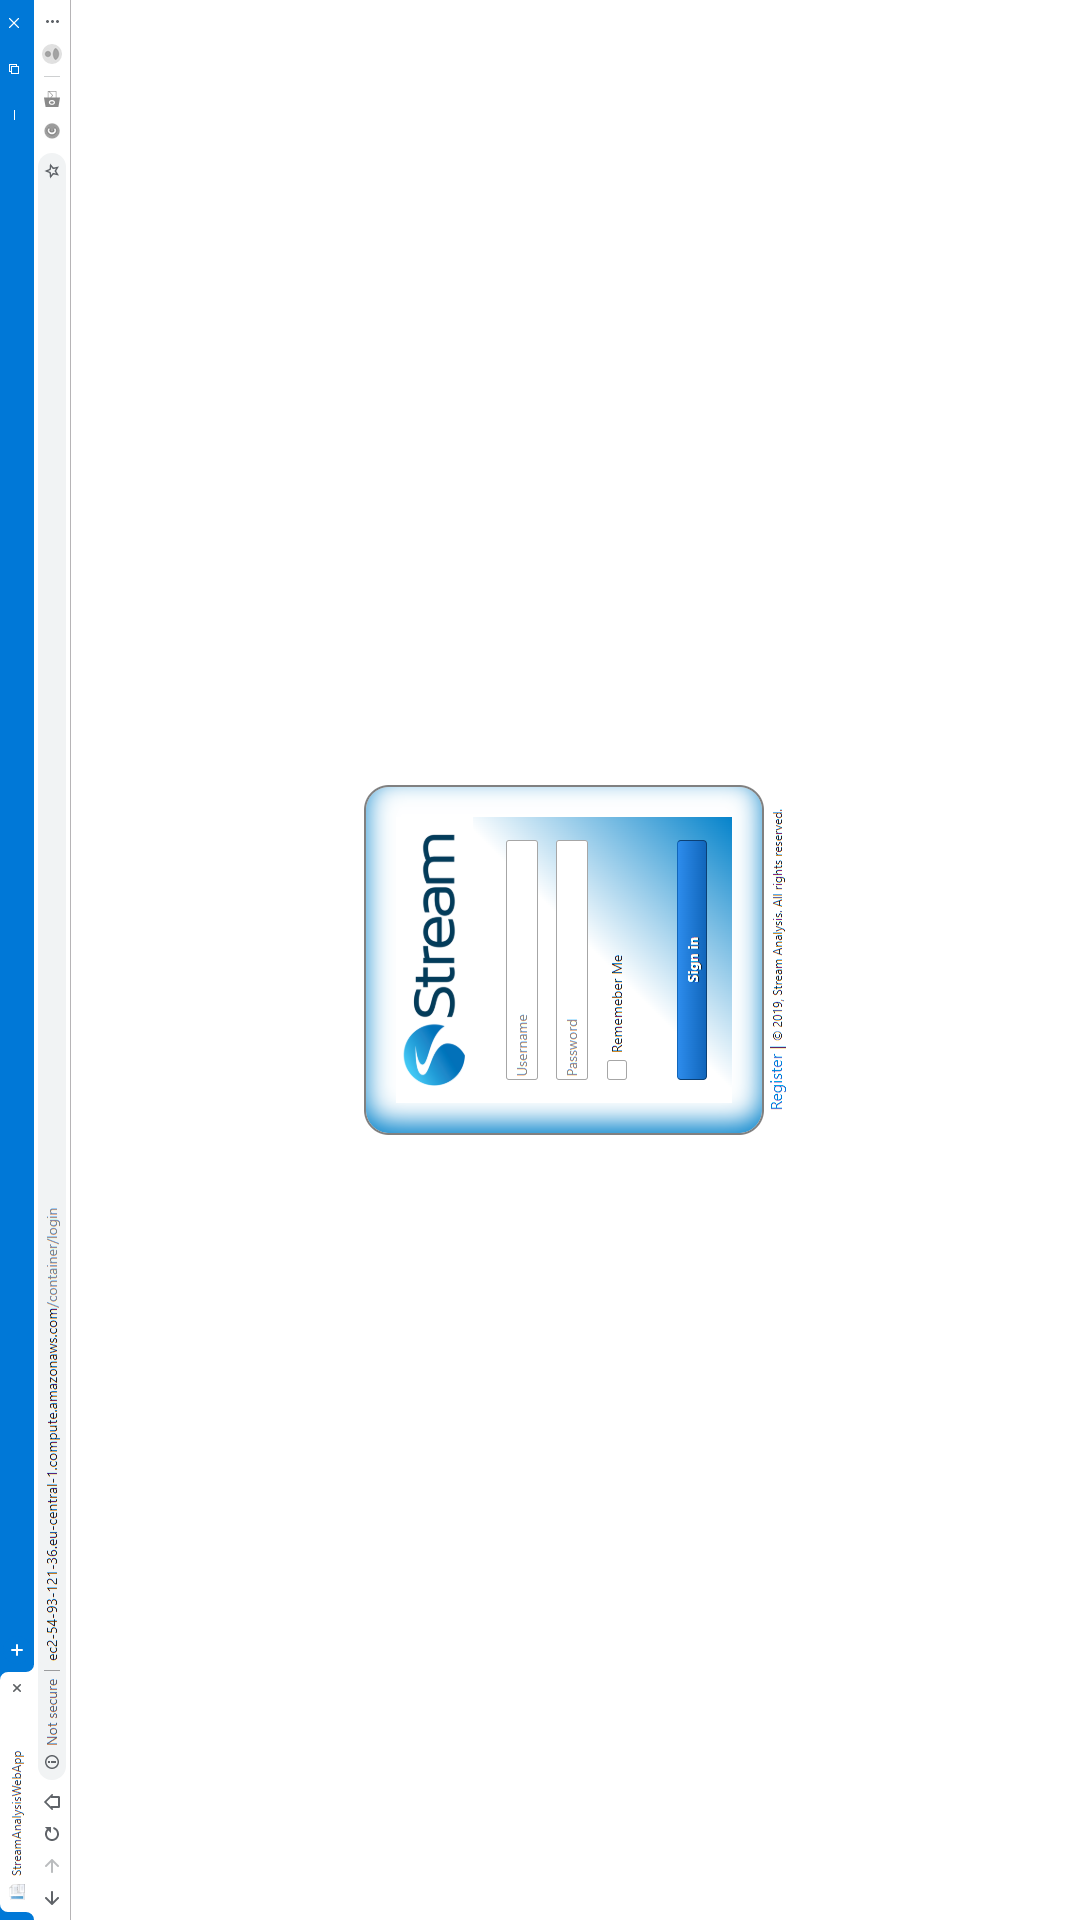
\includegraphics[width=0.5\paperwidth]{./images/guide/container/login.PNG}
	\caption{Container Login Page}
	\label{fig:containerLogin}
\end{figure}

\begin{figure}[p]
	\centering
	\noindent
	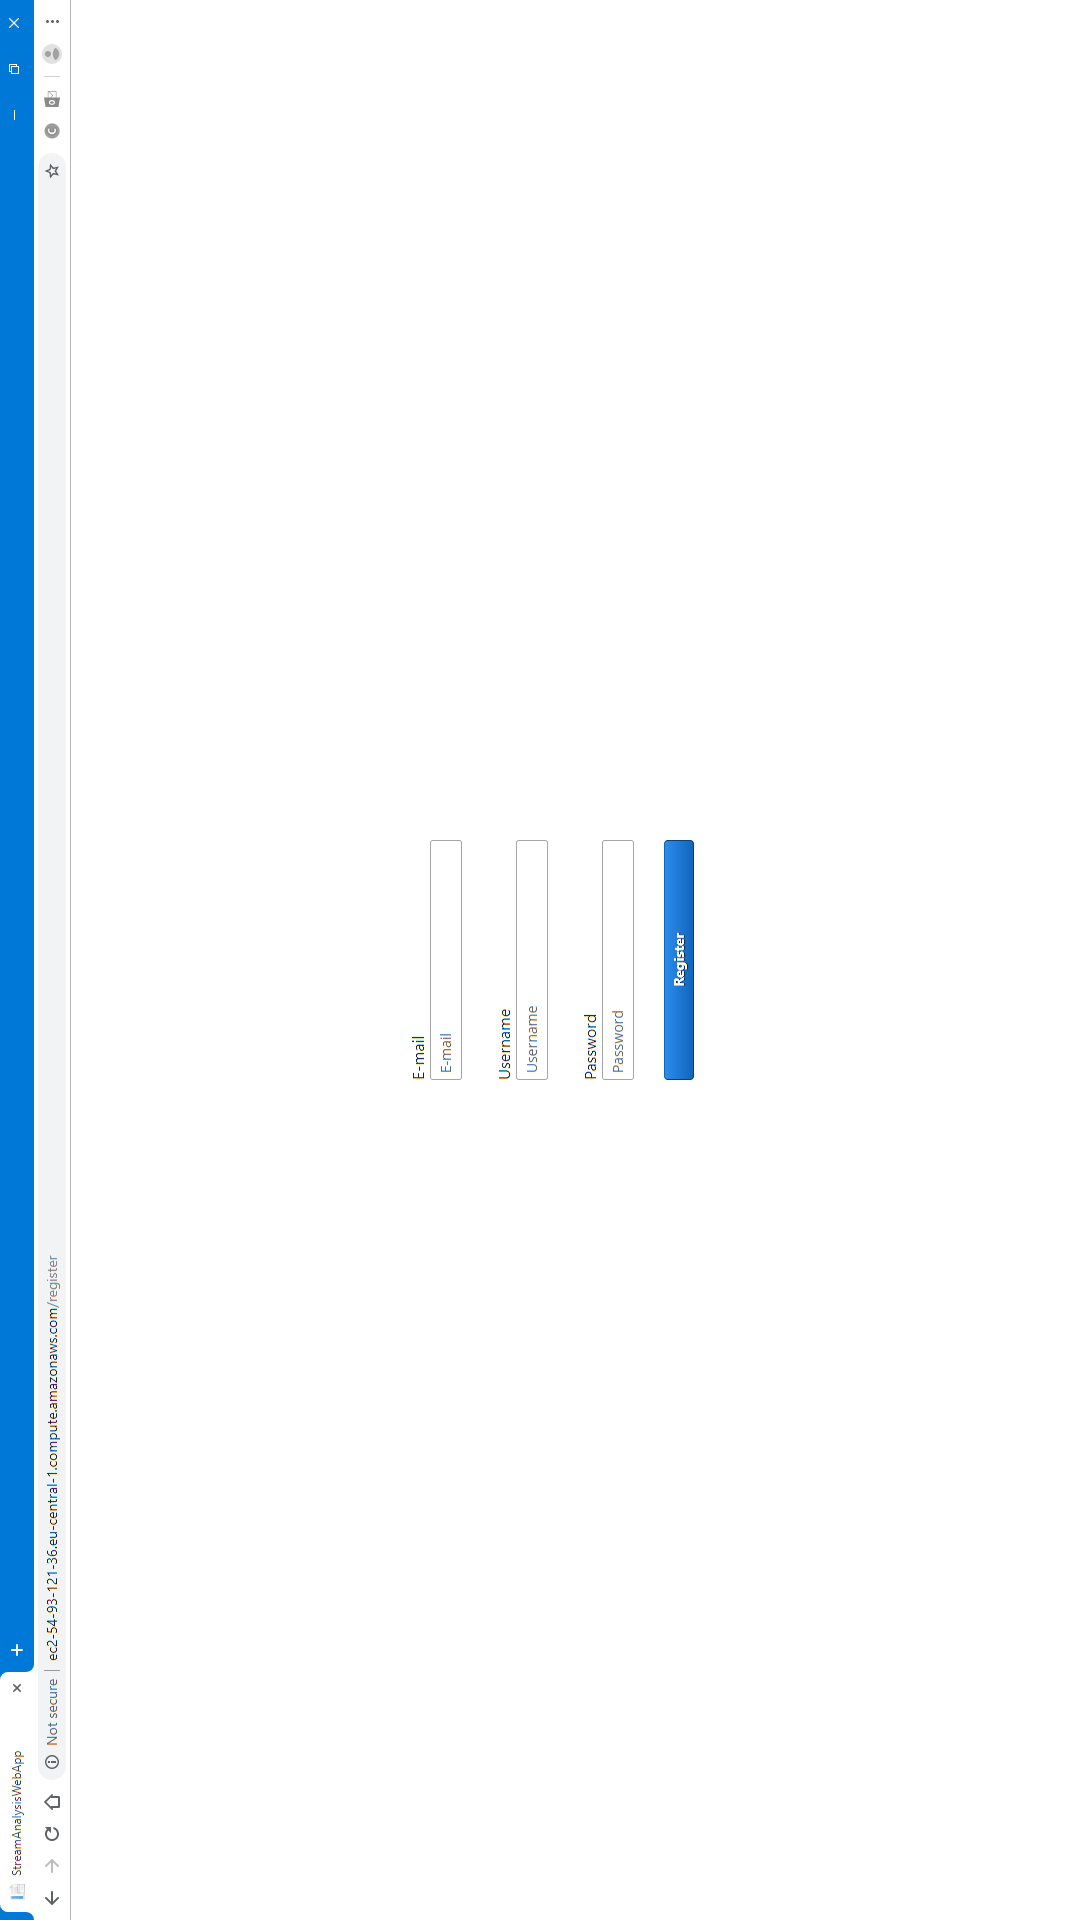
\includegraphics[width=0.5\paperwidth]{./images/guide/container/register.PNG}
	\caption{Container Registration Page}
	\label{fig:containerRegister}
\end{figure}

\begin{figure}[p]
	\centering
	\noindent
	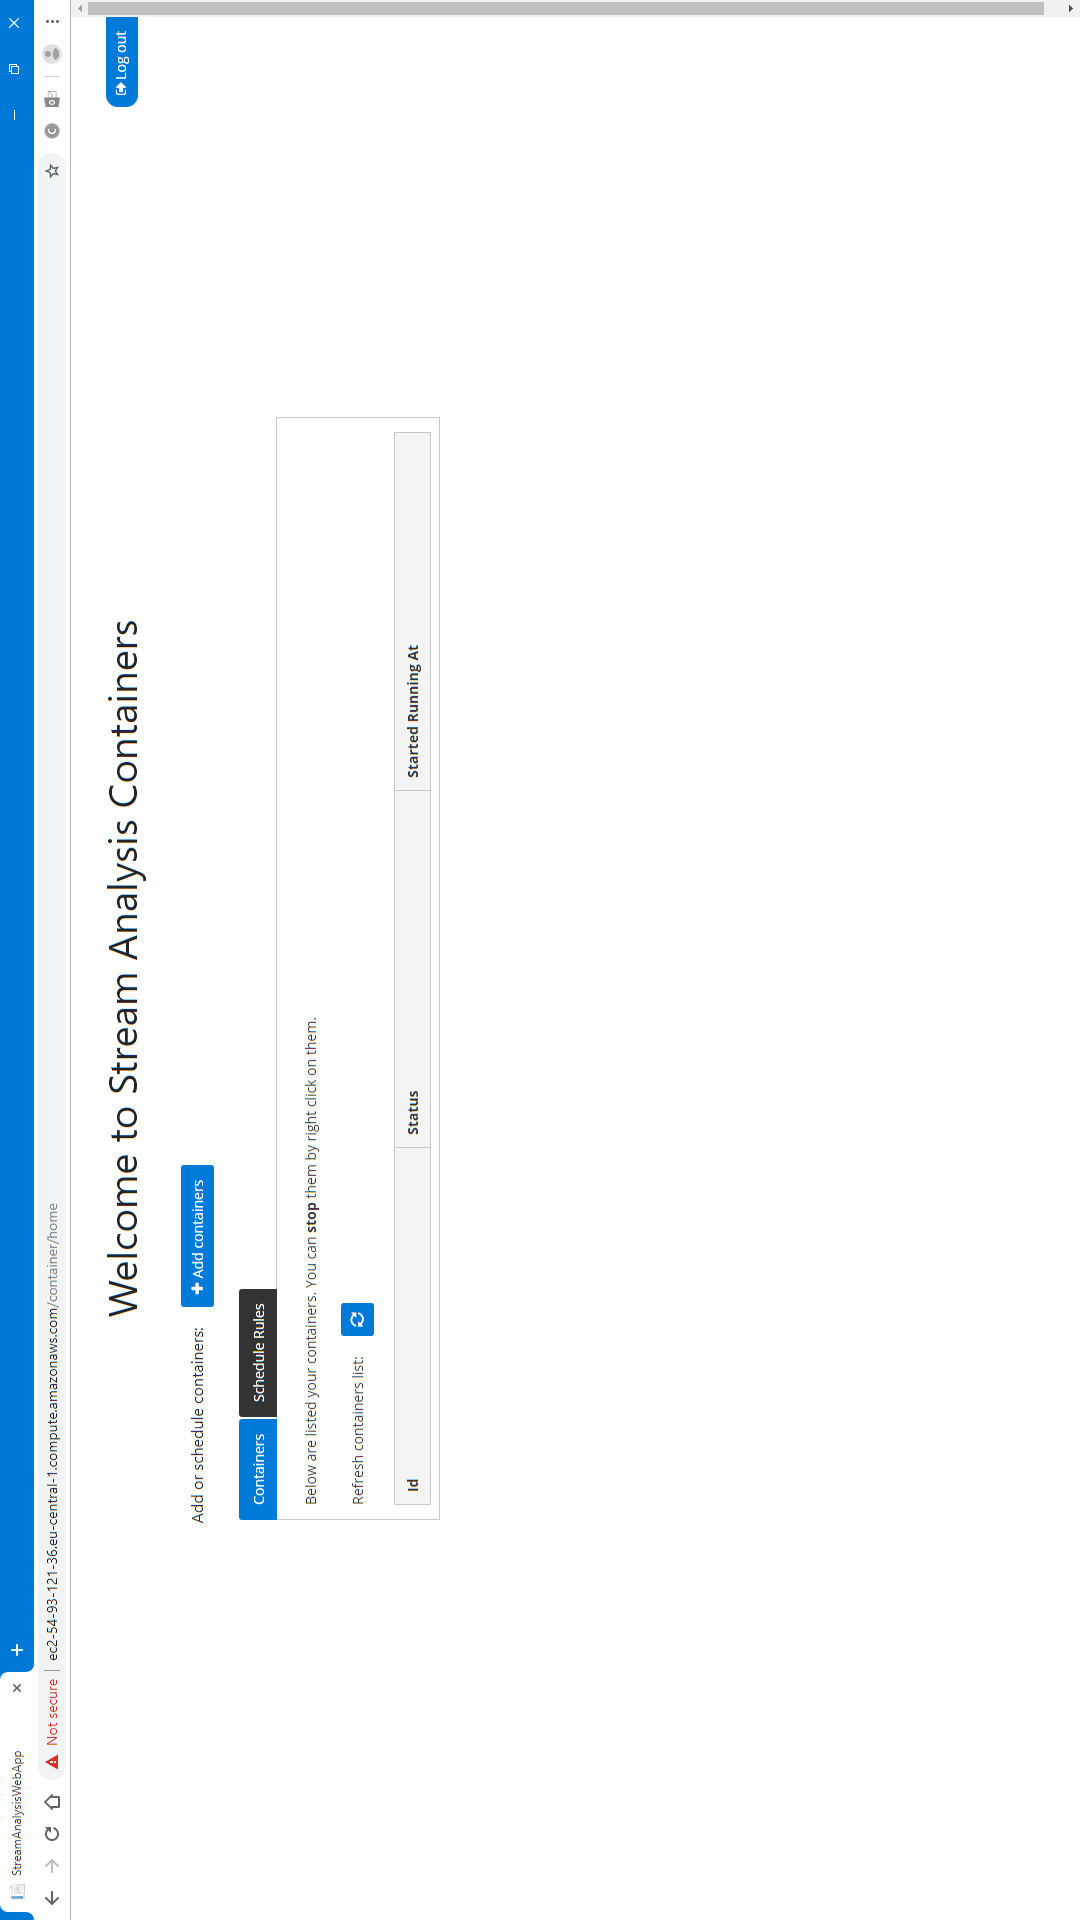
\includegraphics[width=0.5\paperwidth]{./images/guide/container/home.PNG}
	\caption{Container Home Page}
	\label{fig:containerHome}
\end{figure}

The "Add containers" button will route the user to the container creation page, which has the below path. On the top right side there is a button name "Home" which can be used to navigate back to the home page.\\

\textit{http://ec2-54-93-121-36.eu-central-1.compute.amazonaws.com/container/create}\\

The user must pass through all the steps displayed:

\begin{enumerate}
	\item Broker
	\item Repository
	\item Push image
	\item Configure
	\item Run image
\end{enumerate}

\newpage

\subsection{Broker}
\label{chap:05:01:01}

On this page the user can find all the necessary information on to broker IP and how the queue and topic models should look like.

On the other hand he/she can add topics and queues by clicking the buttons "Add topic" and "Add queue". The user must provide names for these channels but when he/she uses them in his containerized application, he/she must prefix them with the provided id followed by a dash.\\

\begin{figure}[p]
	\centering
	\noindent
	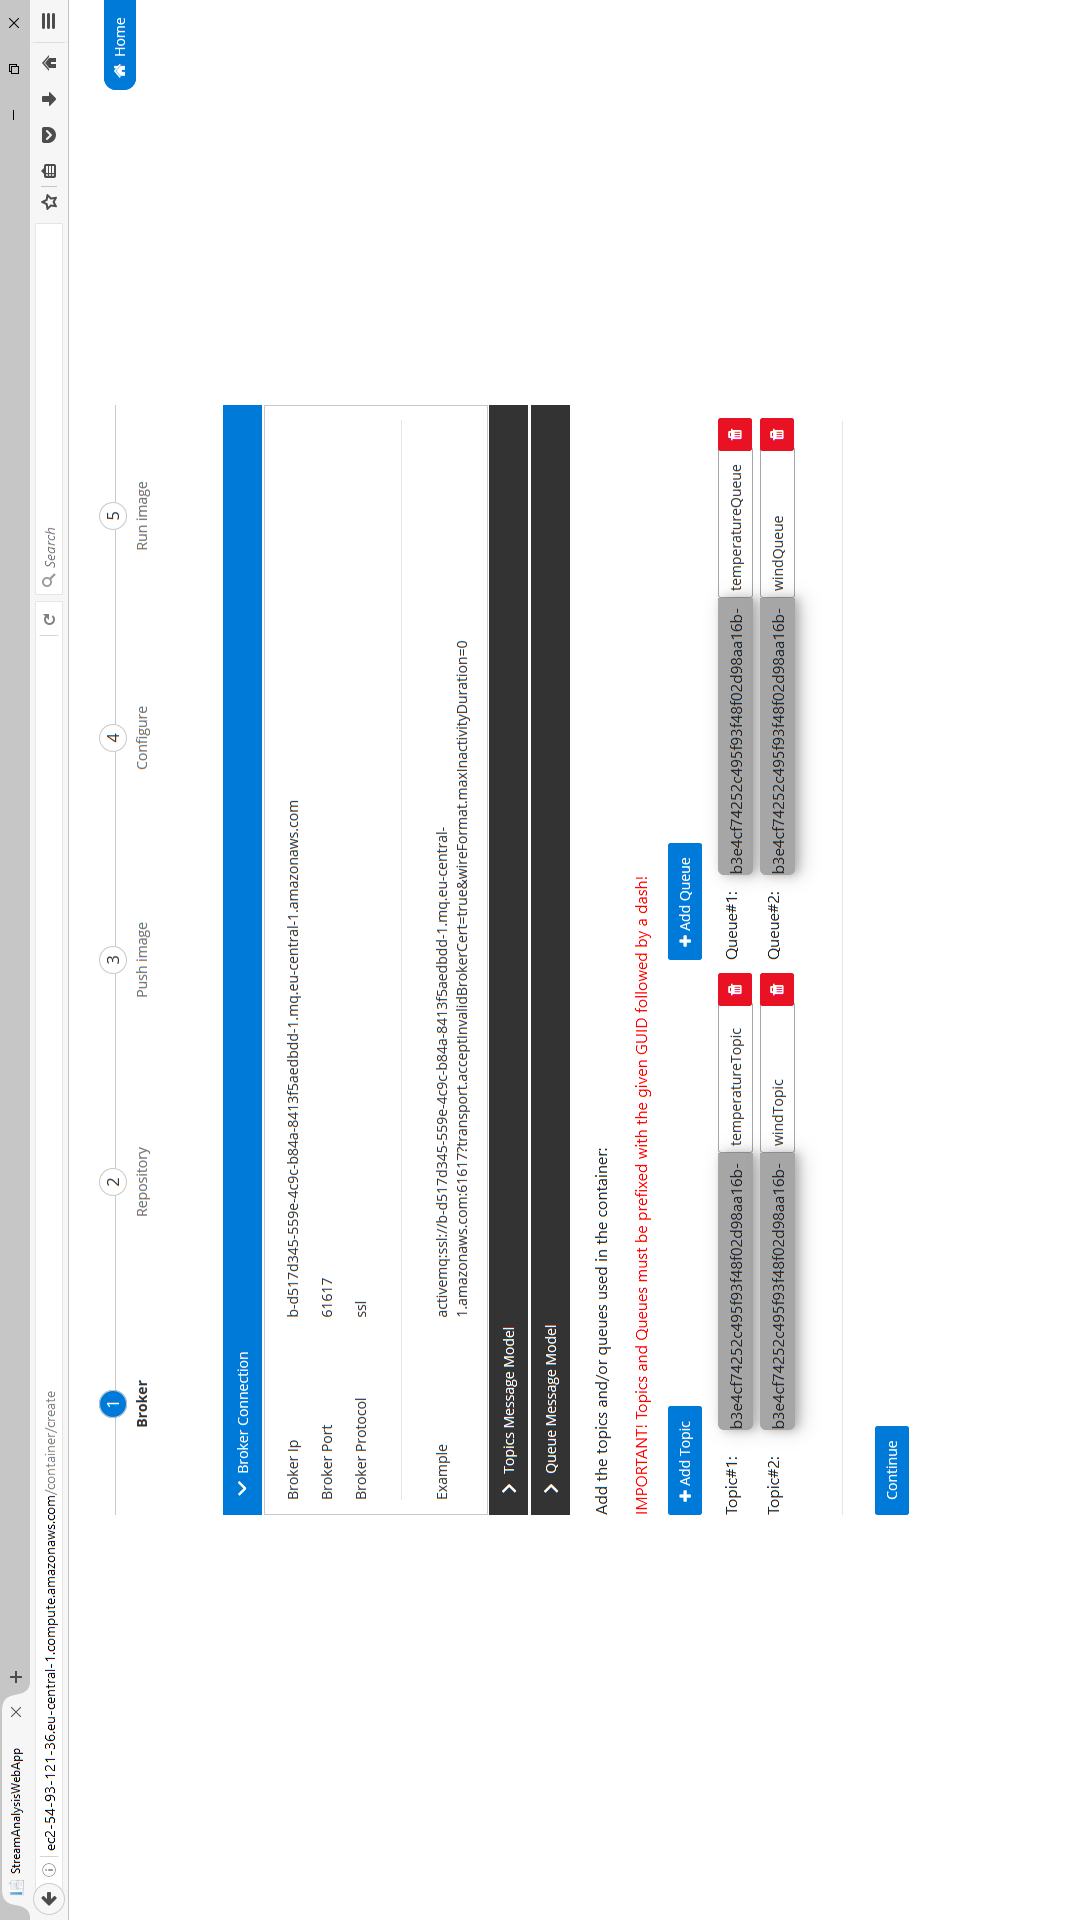
\includegraphics[width=0.5\paperwidth]{./images/guide/container/broker.PNG}
	\caption{Broker Step}
	\label{fig:broker}
\end{figure}

Moving on to the next step by clicking on the "Continue" button the user arrives to the second step.

\newpage

\subsection{Repository}
\label{chap:05:01:02}

\begin{figure}[p]
	\centering
	\noindent
	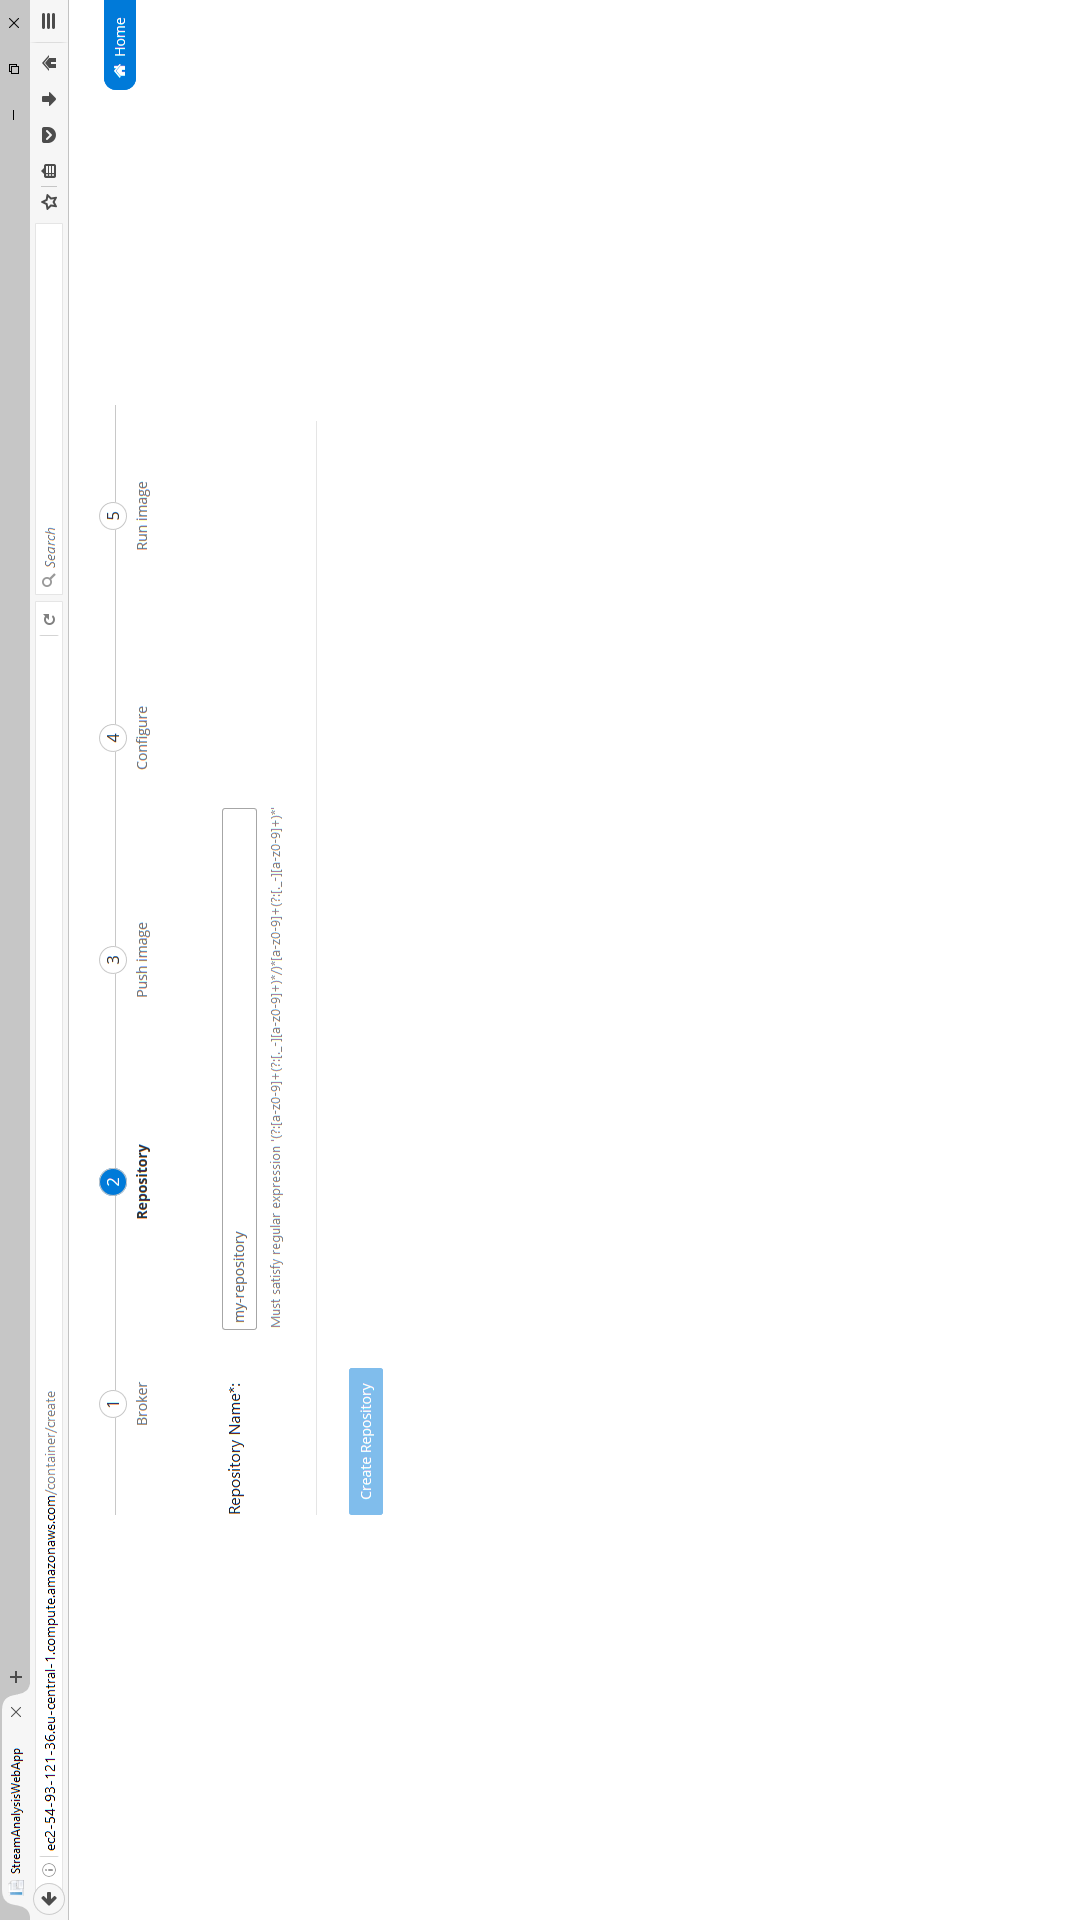
\includegraphics[width=0.5\paperwidth]{./images/guide/container/repository.PNG}
	\caption{Repository Step}
	\label{fig:repository}
\end{figure}

On this step the user has to input a repository name for the image. Once this is done he/she can move forward by clicking on the button "Create Repository". At this stage he/she is shown the Push image step.

\newpage

\subsection{Push Image}
\label{chap:05:01:03}

\begin{figure}[p]
	\centering
	\noindent
	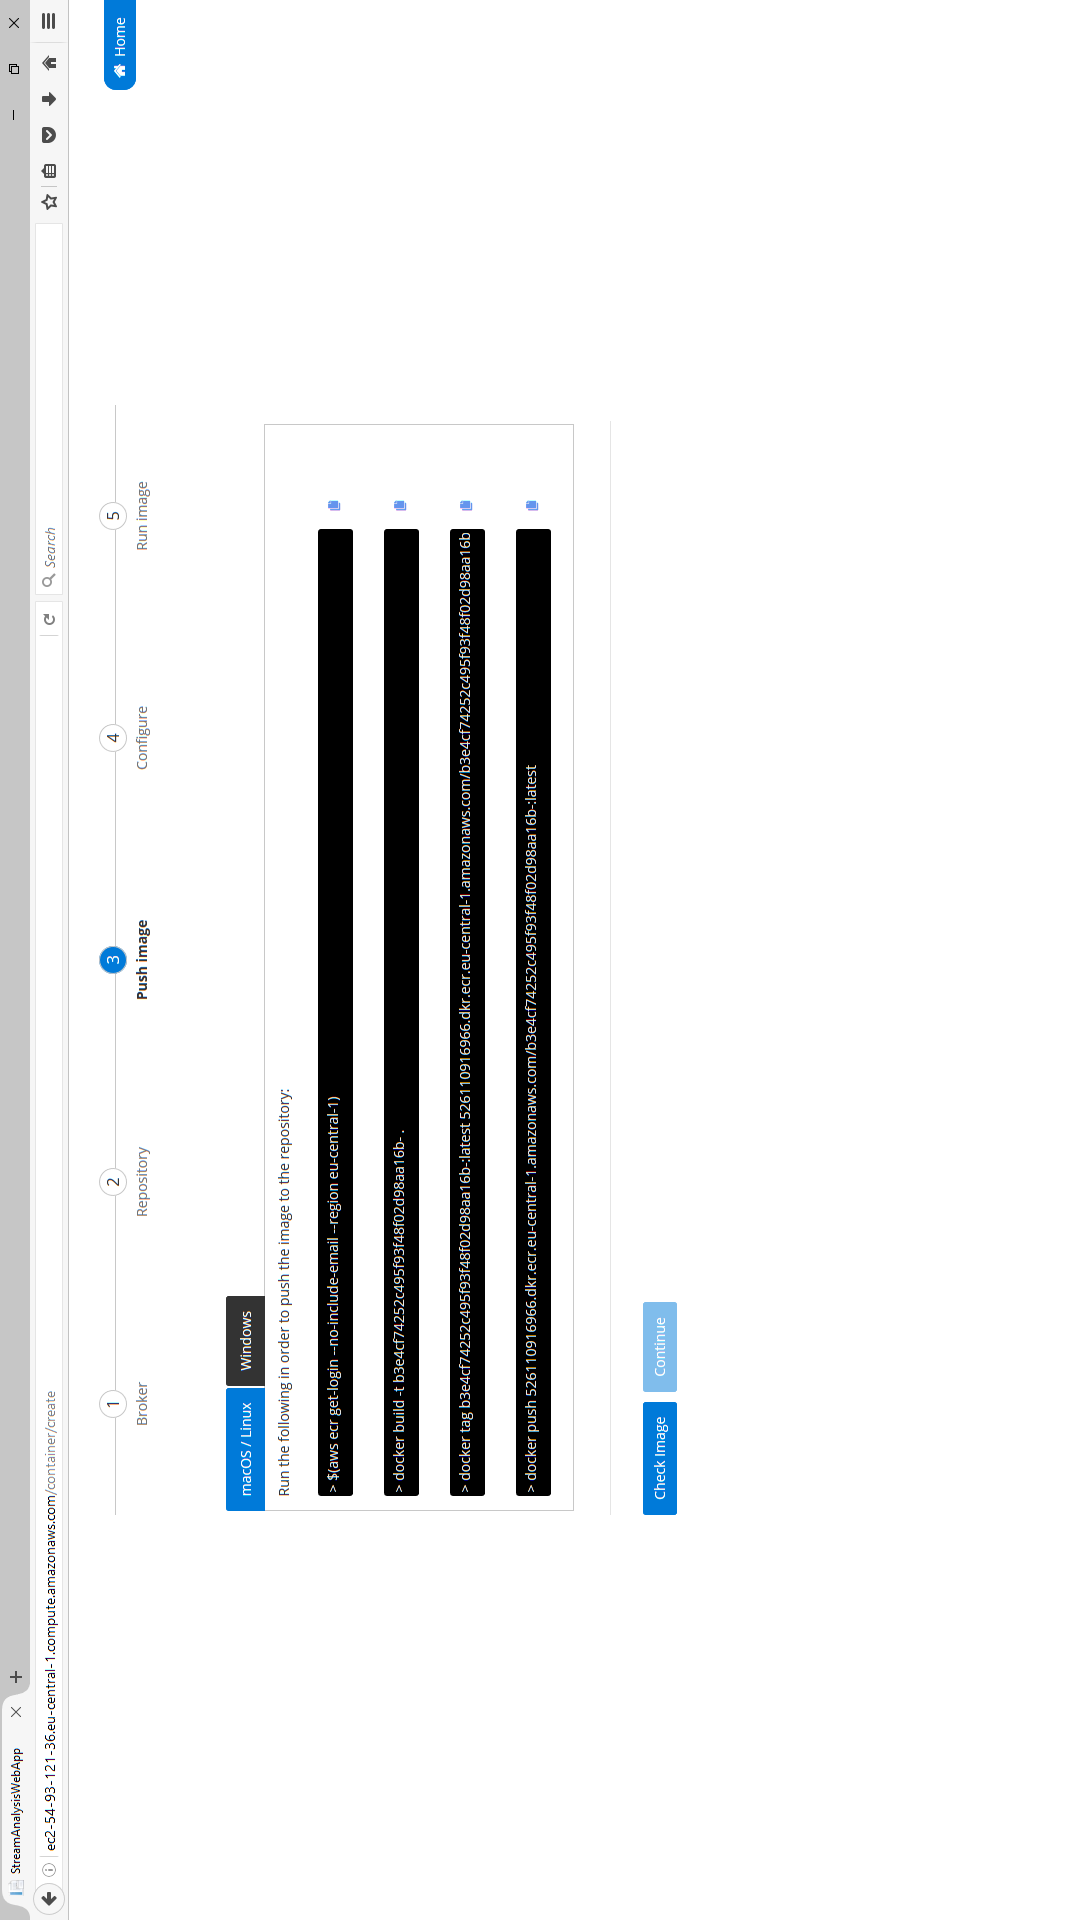
\includegraphics[width=0.5\paperwidth]{./images/guide/container/pushImage.PNG}
	\caption{Push Image Step}
	\label{fig:pushImage}
\end{figure}

Depending on his operating system the user can select from the two tabs the appropriate instruction on how to push the image to the repository. On Windows for example the user needs to open PowerShell and run the commands in order. There are four commands and they do the following: login into the repository from the cloud, build the image, tag the image with the repository and finally push the image to the repository.

He/she then needs to press the button "Check Image" in order to see if the image was successfully uploaded into the cloud. If yes, then the "Continue" button will be enabled and he/she can press it to navigate further to the fourth step which is Configure.

\newpage

\subsection{Configure Image}
\label{chap:05:01:04}

\begin{figure}[p]
	\centering
	\noindent
	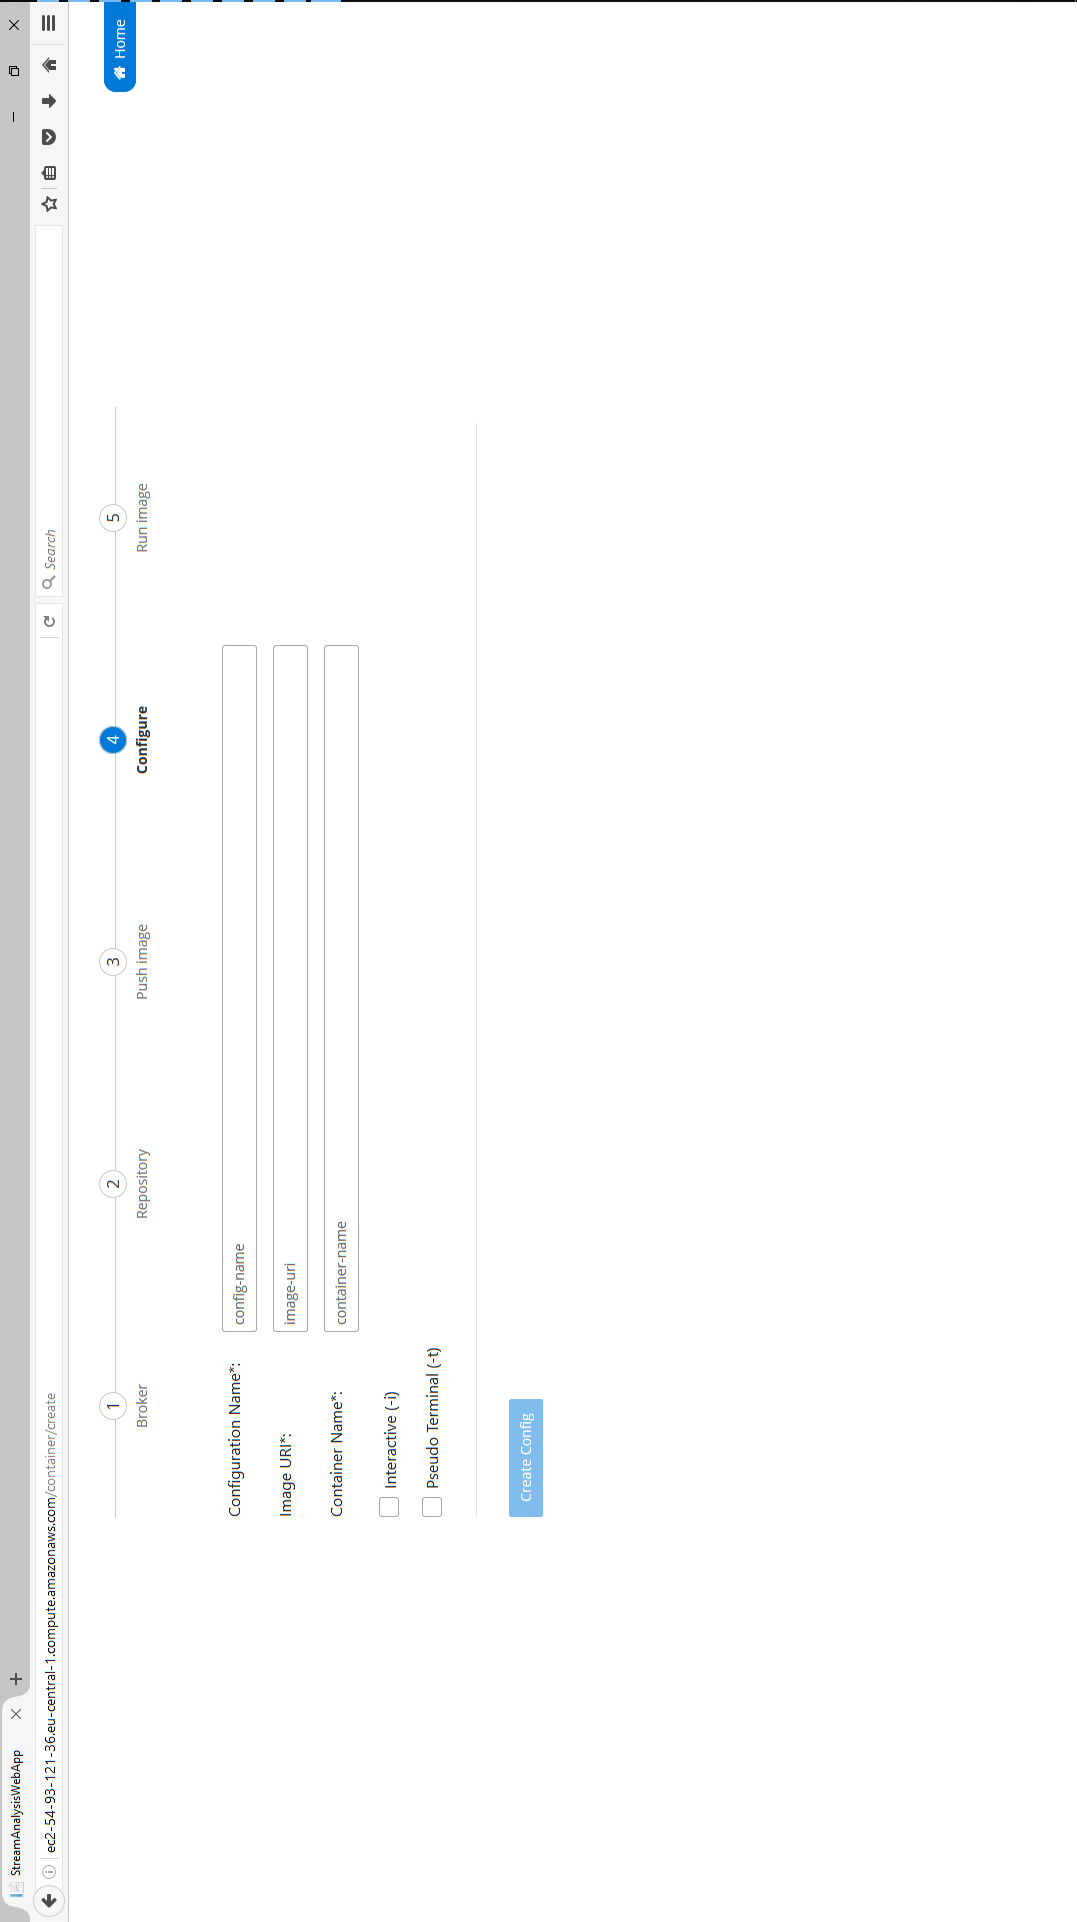
\includegraphics[width=0.5\paperwidth]{./images/guide/container/configure.PNG}
	\caption{Configure Image Step}
	\label{fig:configure}
\end{figure}

The purpose of this step is to create a configuration when the image is ran, hence when the container is created.

The user needs to input the following: a configuration name, the image URI should already be populated, a container name. He/She also has the option to select of the image should run with the interactive or pseudo terminal features. Once this is done he/she can move to the next step by clicking on the button "Create Config".

\newpage

\subsection{Run Image}
\label{chap:05:01:05}

At this stage the user has arrived to the final and most important step: run image.

\begin{figure}[p]
	\centering
	\noindent
	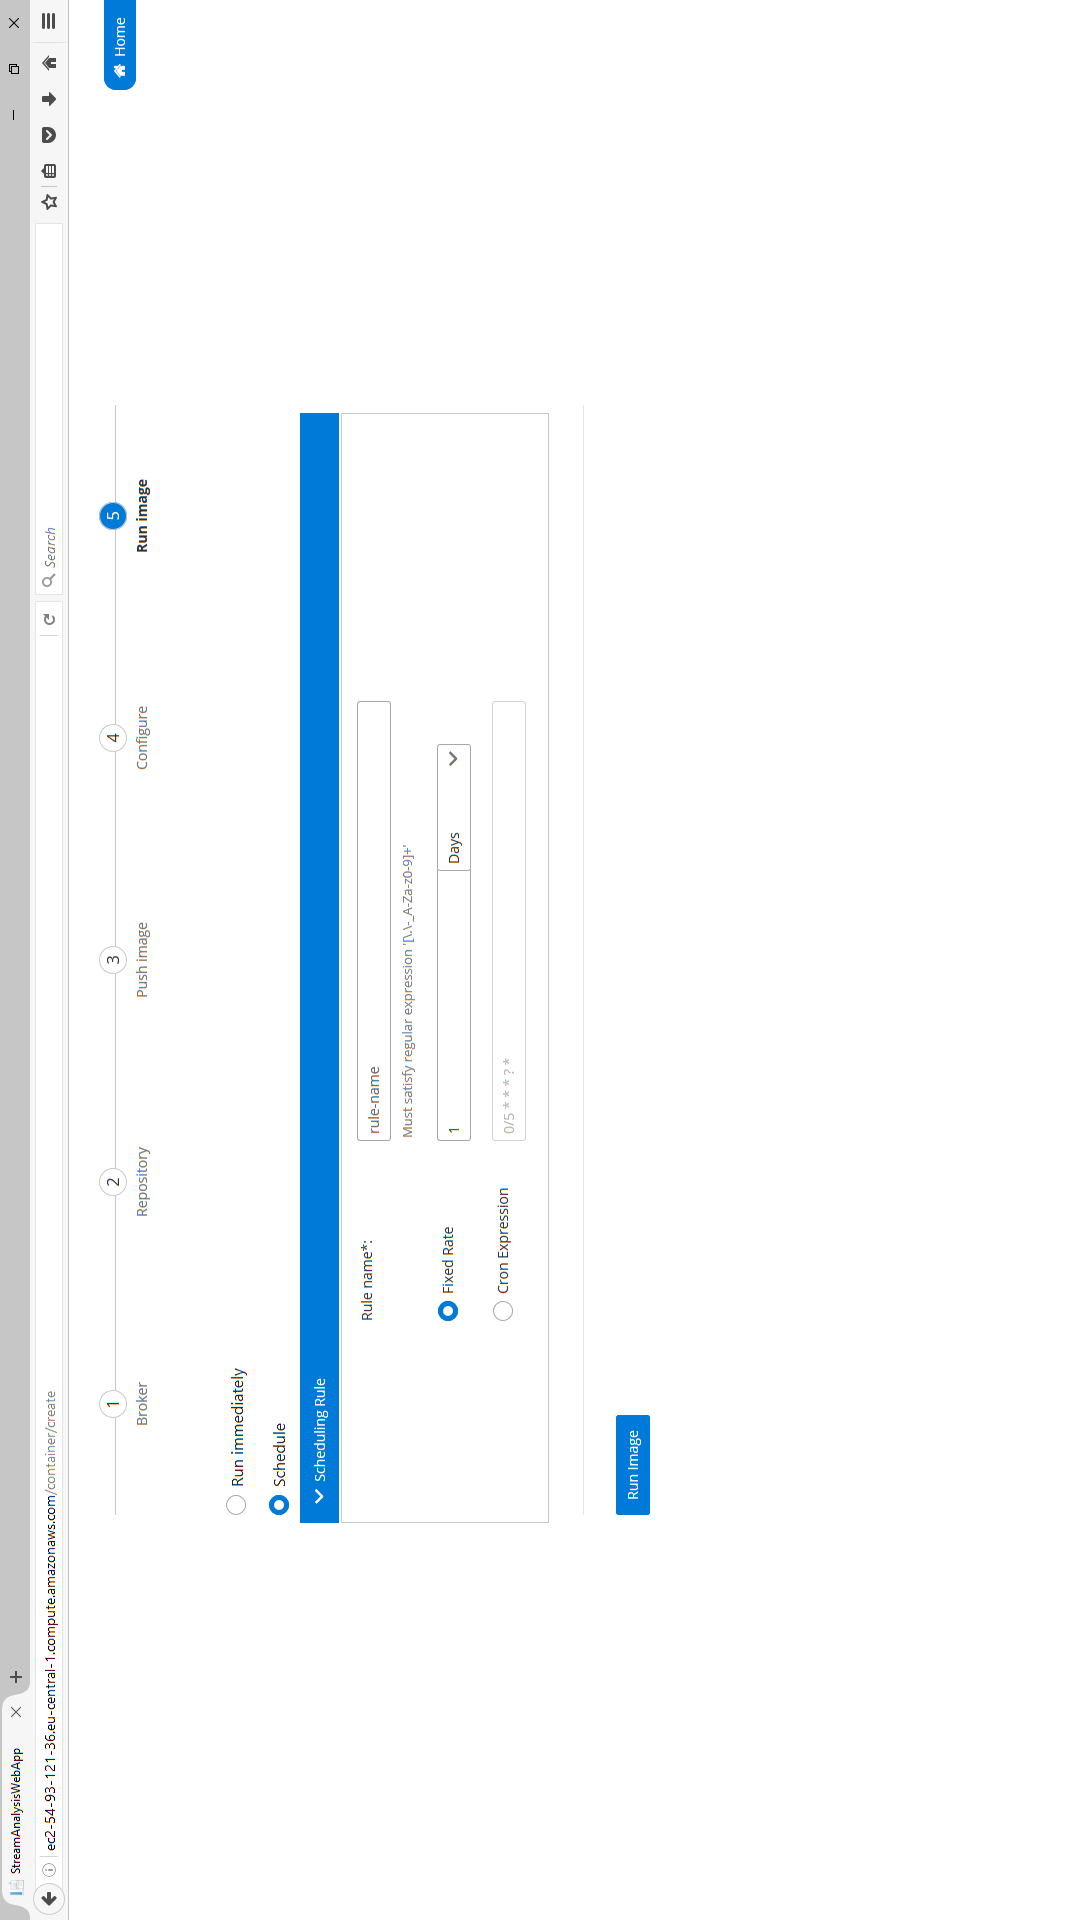
\includegraphics[width=0.5\paperwidth]{./images/guide/container/runImage.PNG}
	\caption{Run Image Step}
	\label{fig:runImage}
\end{figure}

Let's say the user needs to run his container every other day. In this case he/she needs to selected the "Schedule" radio button so that the scheduling panel would appear. He/She then needs to input a scheduling rule name and make sure that the "Fixed Rate" radio button is selected and type in 1 and select Days from the dropdown box.

Finally he/she can press the "Run image" button and confirm that he/she wants to proceed. At this stage the cloud setup will try to launch the a container from the provided image. Note that this process takes a few minutes.

The Front-end provides a mechanism to track all the user's launched containers on the home page. Their status is shown which can be pending or running as shown in figure \ref{fig:containersExample}. Note that by right clicking on one of the containers, the users can stop them and then start them again with ease as seen in figure \ref{fig:runningContainer}.\\

\begin{figure}[p]
	\centering
	\noindent
	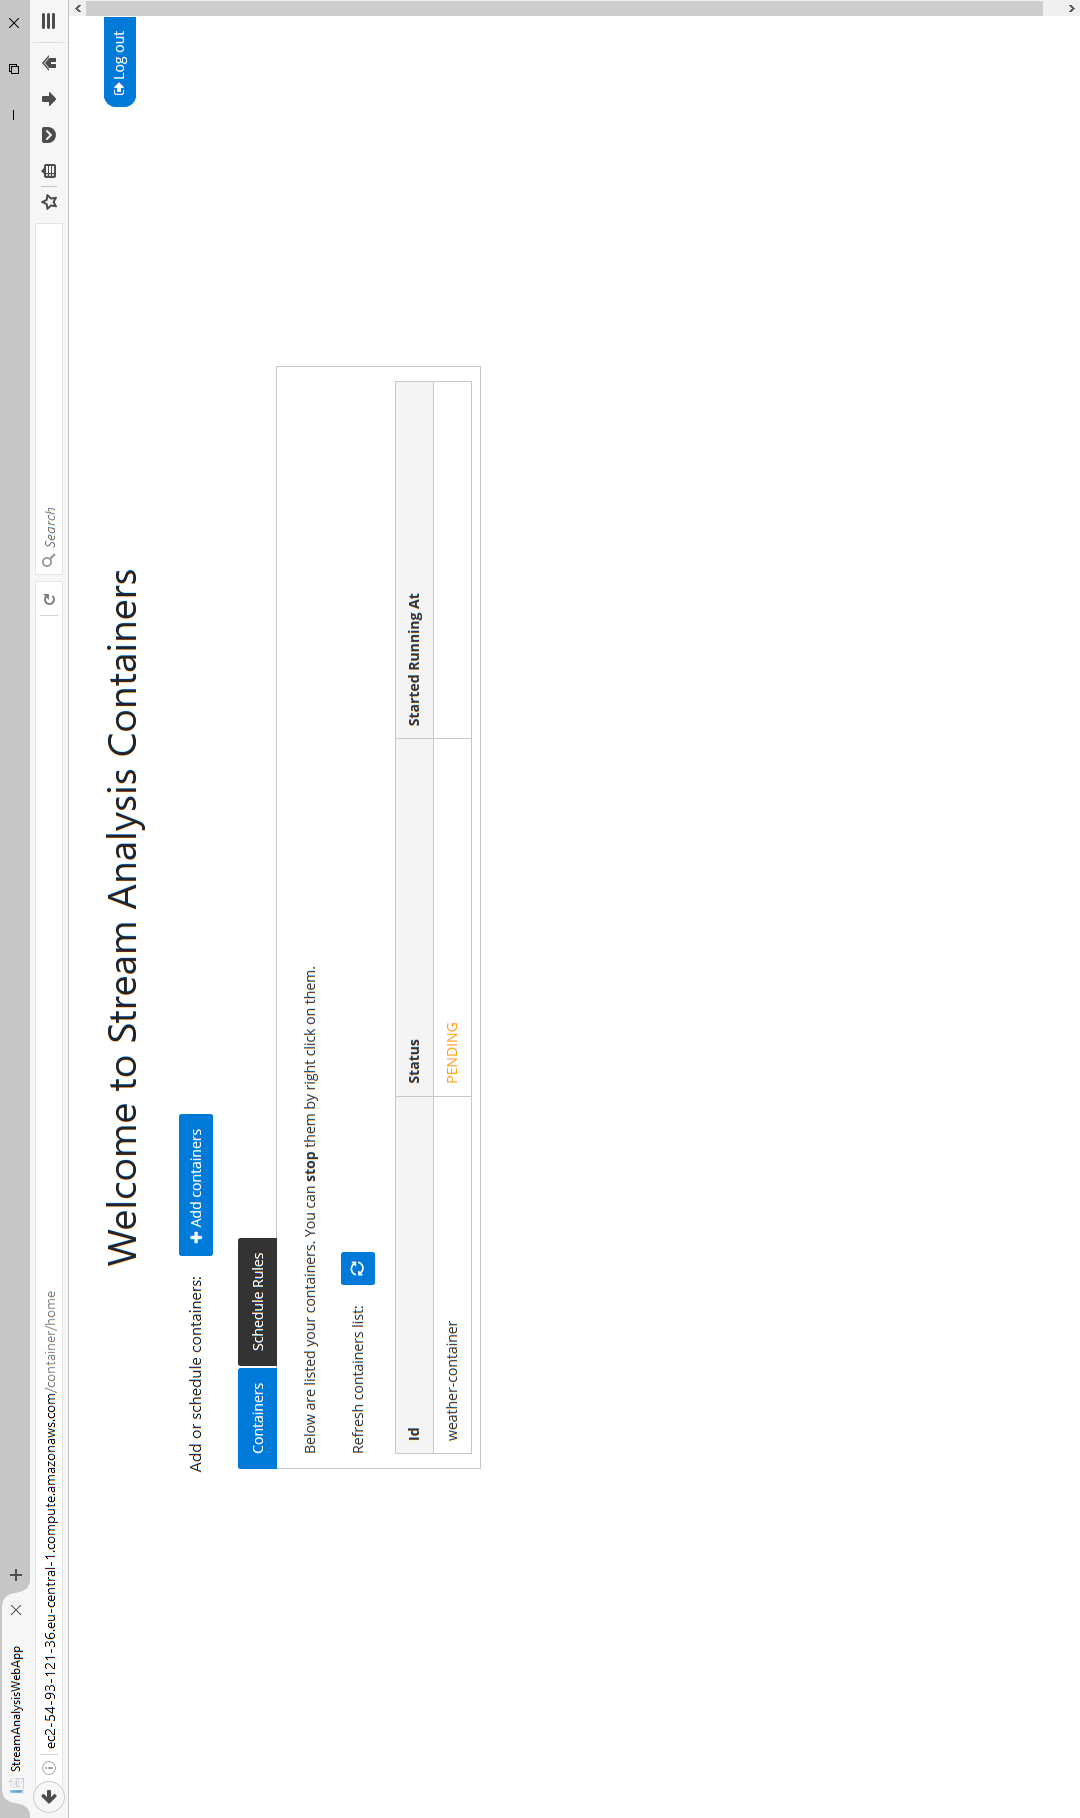
\includegraphics[width=0.5\paperwidth]{./images/guide/container/containersExample.PNG}
	\caption{Container Status}
	\label{fig:containersExample}
\end{figure}

\begin{figure}[p]
	\centering
	\noindent
	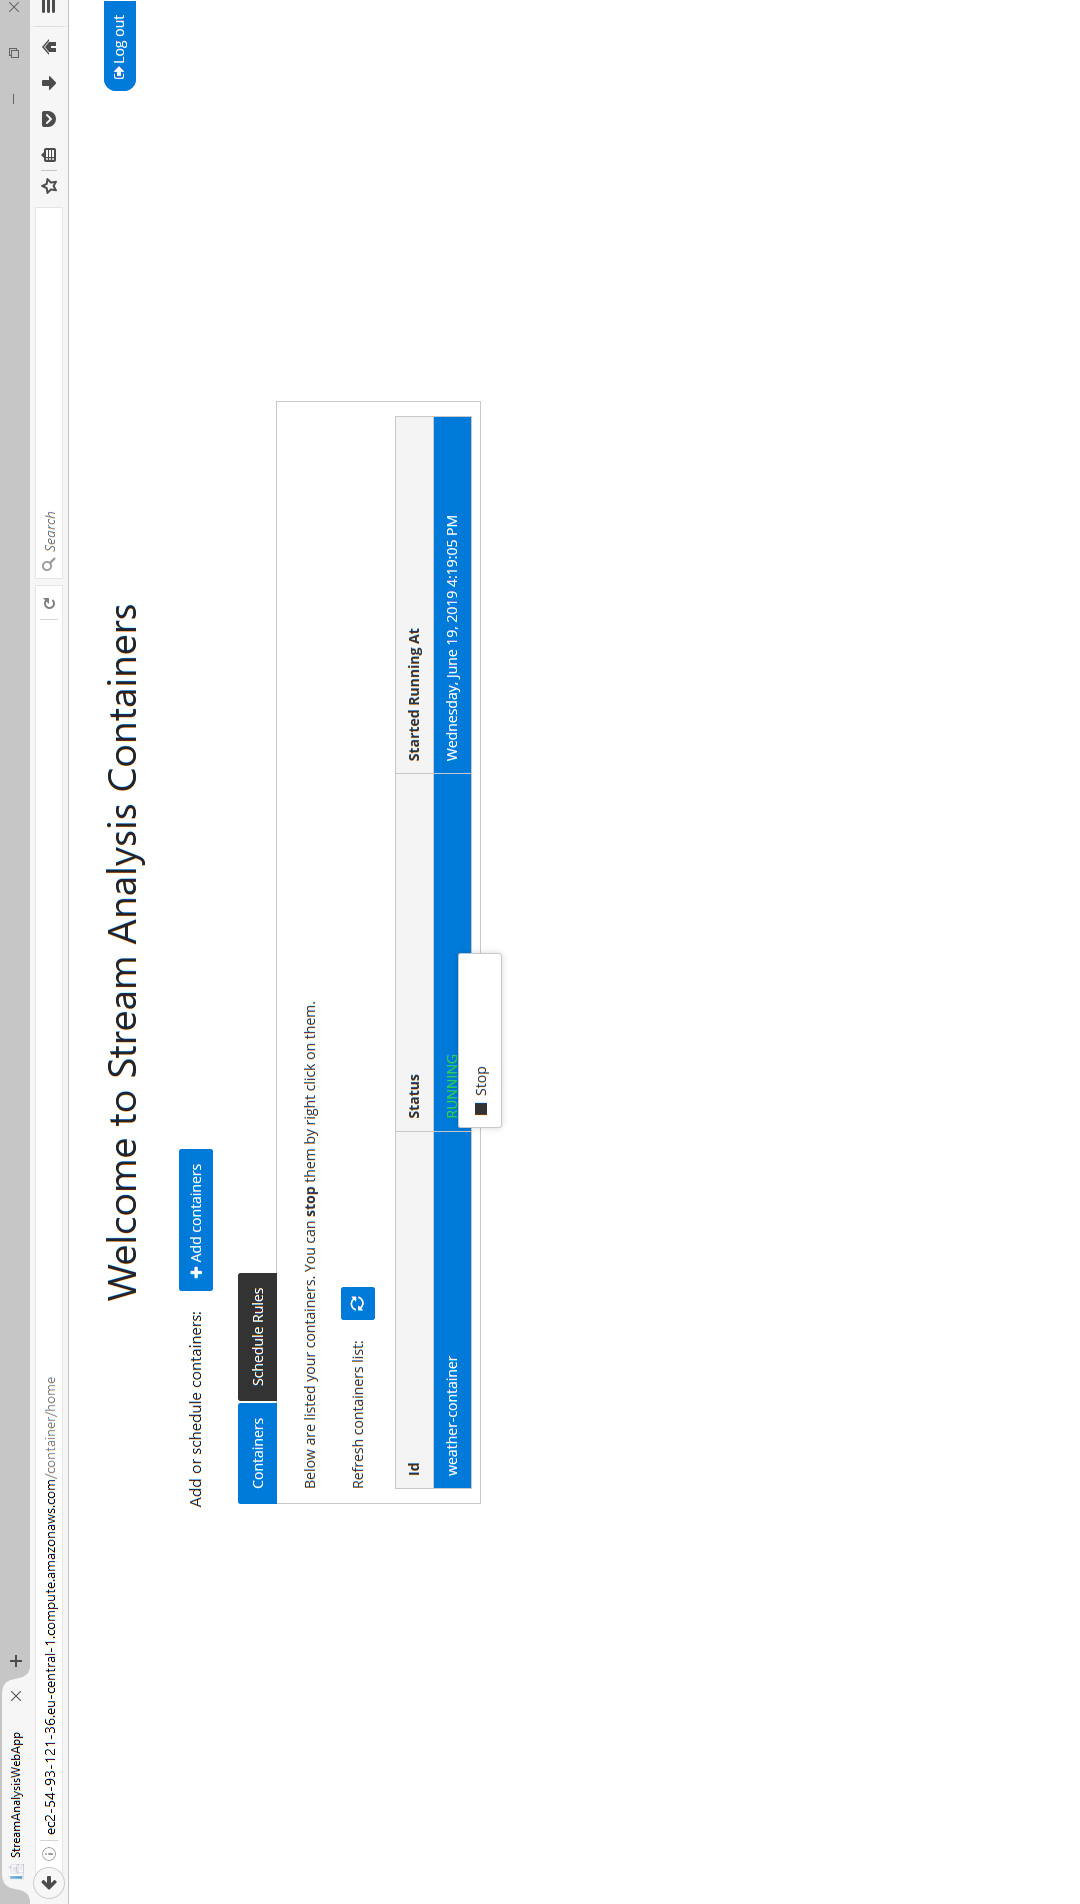
\includegraphics[width=0.5\paperwidth]{./images/guide/container/runningContainer.PNG}
	\caption{Running Container}
	\label{fig:runningContainer}
\end{figure}

\newpage

\section{Dashboard User}
\label{chap:05:02}

The dashboard user needs to login the same way as the containerized application user, however he/she has other path for the login page.\\

\textit{http://ec2-54-93-121-36.eu-central-1.compute.amazonaws.com/login}\\

Once he/she is successfully logged in, he/she lands on the dashboard page.

\begin{figure}[p]
	\centering
	\noindent
	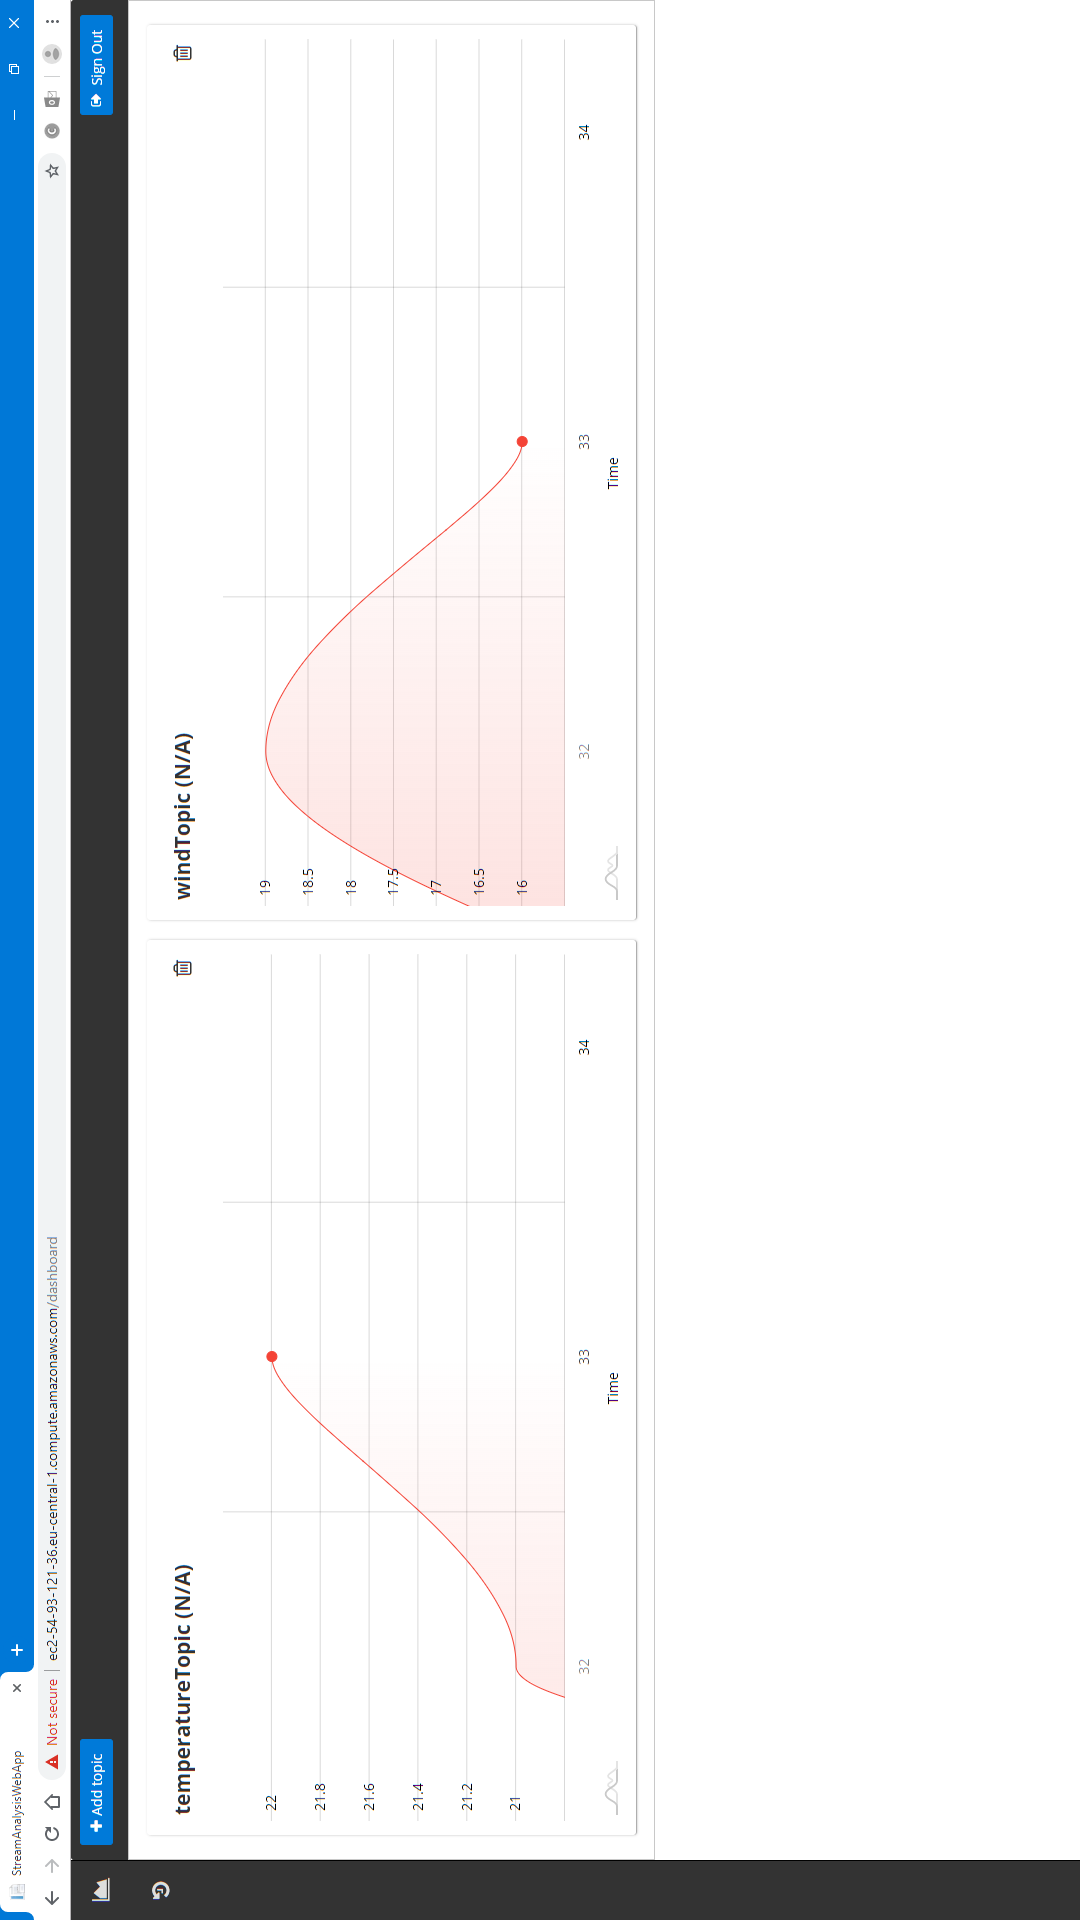
\includegraphics[width=0.5\paperwidth]{./images/guide/dashboard/dashboard.PNG}
	\caption{Dashboard Page}
	\label{fig:dashboard}
\end{figure}

On the dashboard page he/she can click on the "Add topic" button in order to listen to topic messages. Once the desired topics are added the charts will be shown. These are real time based charts where on data arrival the chart updates itself.

From the left side menu the user can select the "Historical" option which will route him to the historical page at:\\

\textit{http://ec2-54-93-121-36.eu-central-1.compute.amazonaws.com/historical}\\

\begin{figure}[p]
	\centering
	\noindent
	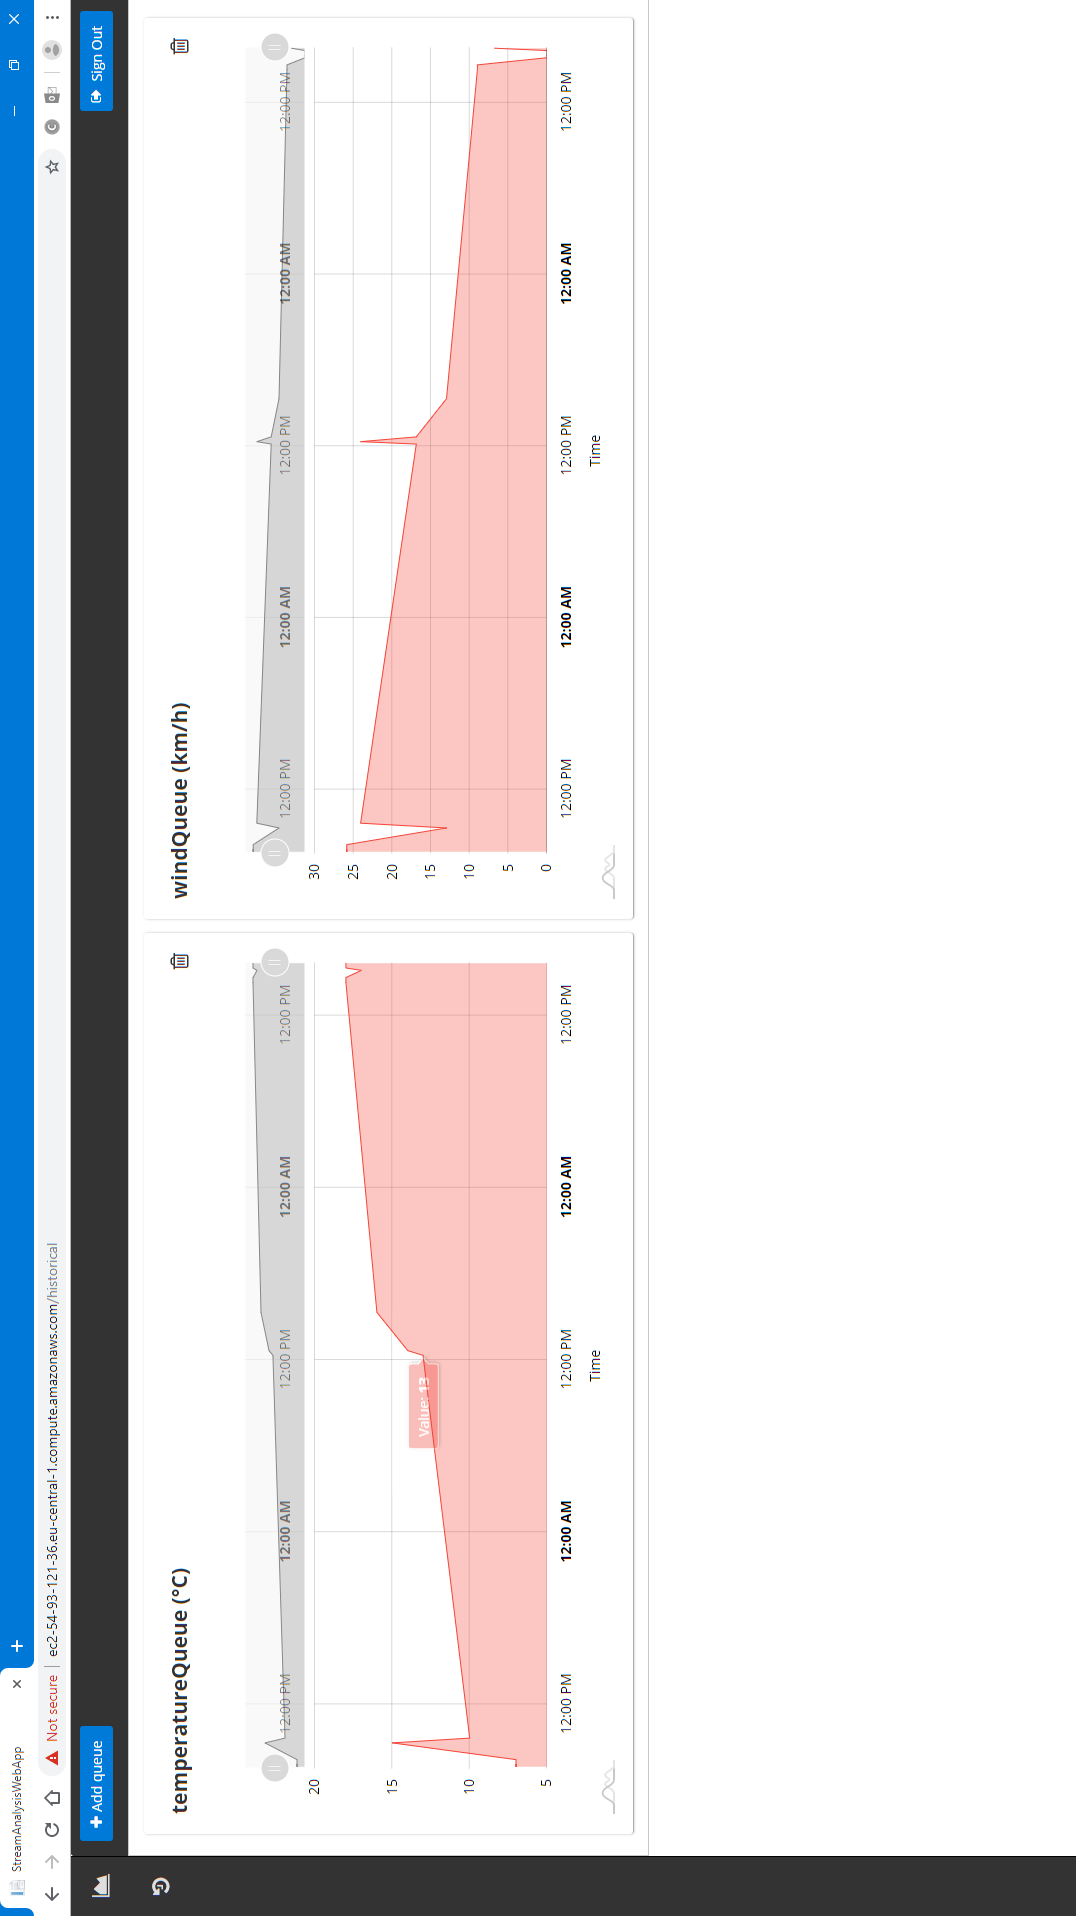
\includegraphics[width=0.5\paperwidth]{./images/guide/dashboard/historical.PNG}
	\caption{Historical Page}
	\label{fig:historical}
\end{figure}

On the same was as the topics were added, the user can click on the "Add queue" button and select the desired queues to be plotted.
